\graphicspath{{./main/2_introduction/figures/}}

\chapter{Introduction}
\label{chap:intro}

Every single organism in an ecosystem has the property to have a life-form. Humans, as many of the other species organisms, are part of the biological evolution. Darwin states in~\citep{darwin1859} that all species of organisms arise and develop through the natural selection of small, inherited variations that increase the individuals ability to compete, survive, and reproduce. As individual organisms, we are responsible to observe, plan and execute a series of actions that will determine the interaction with our surrounding environment. The capability of communicating with other individuals, move from one place to the other, or search and grasp objects are just examples of primitive actions that help us to interact with our environment. However, in order to perform many of those primitive actions it is needed to have and use a perception system in order to gather and interpret sensory information. As humans, our perception system can be extremely complex and composed by several layers of sensory cells that respond to a specific type of physical stimulus which eventually will be processed by our brains and used to perform specific actions.

The human perception system evolved such in a way that reconstructs our environment and intrinsically creates an internal representation to assure this interaction and eventually make us as specie to survive. In this direction, the main motivation of this work is to study the different mechanisms that the human perception system uses to reconstruct the environment and bridge it with computer vision. Precisely, in this thesis we first study the problem of scene reconstruction - understood as a sequential pipeline, we review the existing solutions and propose new methods for two of the main tasks in classical multi-view scene reconstruction: key-point detection and key-point description. With this aim, in this thesis we have develop a new Python library (Kornia) that fills the gap between classical computer vision systems and current deep learning based approaches. Using this library a multi-camera scene reconstruction systems has been built, which is the last contribution in this thesis.

\section{Scene Reconstruction}

\begin{figure}[t!]
	\centering
	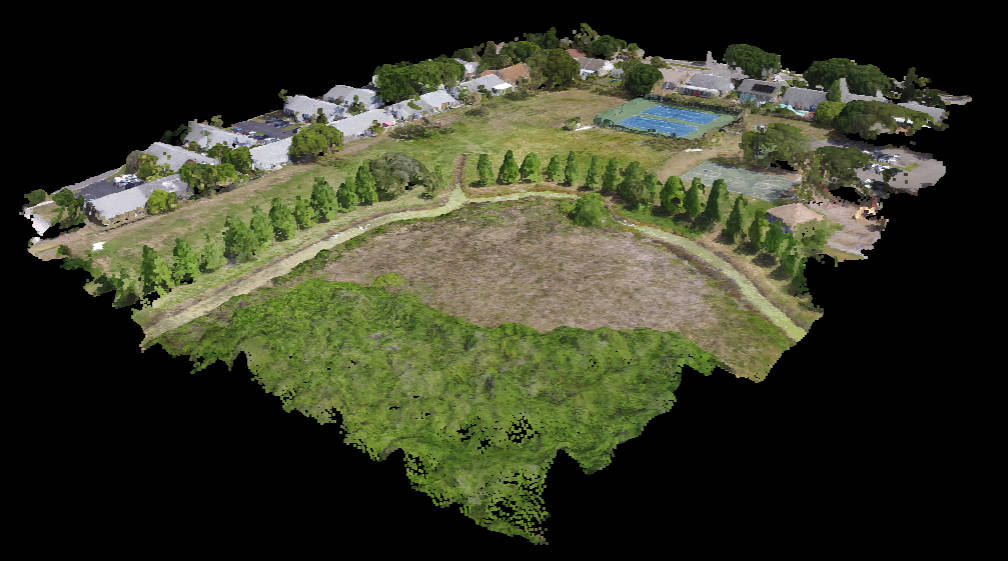
\includegraphics[width=\textwidth]{main/introduction/images/odm_reconstruction.jpg}
	\caption[Result obtained from a complete scene reconstruction pipeline]{\textbf{Result obtained from a complete scene reconstruction pipeline.} Reconstruction obtained using \textit{Open Drone Maps} an open source photogrammetry toolkit to process aerial imagery into maps and 3D models. As can be seen, the global structure of the scene is very accurate after the combination of several computer vision techniques and multi-view geometry. }
	\label{fig:intro_odm_reconstruction}
\end{figure}

In the previous section we introduced the concept of Computer Vision and we associated it to the process to reconstruct a scene similarly as the human perception system does. However, we would like first ask ourselves the following question - \textit{How much related is Computer Vision to the task of scene reconstruction ?} To answer this question, we should first define the problem. Formally, in computer vision and computer graphics, scene reconstruction or 3D reconstruction is the process of capturing the shape and appearance of real object, accomplished either by active or passive methods~\cite{moons2009}. In figure~\ref{fig:intro_odm_reconstruction} we can appreciate the resulting reconstruction of a scene combining several computer vision techniques and multi-view geometry. 

There is an extensive literature about 3D reconstruction describing the  different methodologies and algorithms to solve the entire problem. Nevertheless, the scope of this thesis is to not a give an exhaustive review of the state of the art for all the existing approaches, yet we emphasize specific tasks in chapters~\ref{chap:chap_02}, \ref{chap:chap_03} and \ref{chap:chap_05}. In the next sections, we aim to describe some of the most known approximations for solving the 3D reconstruction problem based on the following approaches: camera pose estimation for two-view image matching, stereo systems, range imaging with RGB-D cameras, and monocular depth estimation for multi-view geometry.

% To answer this question, we can first describe Computer Vision as a sub-field of Computer Science that tries to mimic the human visual system using computers in order to extract and analyse high-dimensional data from digital images or videos from the real world. Computer Vision is an interdisciplinary scientific field related to artificial systems and sometimes referred as, or part of the so known term Artificial Intelligence (AI) that aims to extract information from any kind of images. The type of images can vary depending on the scope of the application and can take many different forms such as single monocular images, video sequences, images from multiple cameras or multi-dimensional data from 3D scanners or medical scanning devices. Besides the types of images that can be acquired, Computer Vision can lead to a wide variety of high level applications including event detection, video tracking, object recognition, 3D pose estimation, motion estimation, visual servoing, 3D scene modeling, image restoration or scene reconstruction.

% As previously discussed, humans have the inherited ability to learn to create abstract representations of our environment that later can be used to perform more complex actions. In our modern era, where everything is automated, we can ask ourselves the following question - \textit{How can we make computers to reconstruct scenes seamless as we humans do ?} A possible answer to this question would be combining the human knowledge with the use of classical and advanced Geometric Computer Vision Techniques. In the field of Computer Vision, Scene reconstruction can be described as the process of creating a virtual representation of a real world entity from data obtained from different sensors such as images or scans.

% There is a lot of literature around how to perform scene reconstruction in computer vision using as a main resource images. Scene reconstruction can be used in many fields such as Robotics, Medicine, Augmented reality, Archaeology, or 3D object recognition, among others. However, in order to solve the task will be very depending on the application and the type of sensors that will be used during the setup design. As we described, scene reconstruction can be defined in a sequential pipeline and approached in many ways. In the following sections we will focus on explaining the reconstruction pipeline from the perspective of local features and later in an end to end manner.

% \begin{figure}
% 	\centering
%     \begin{tabular}{c}
%     	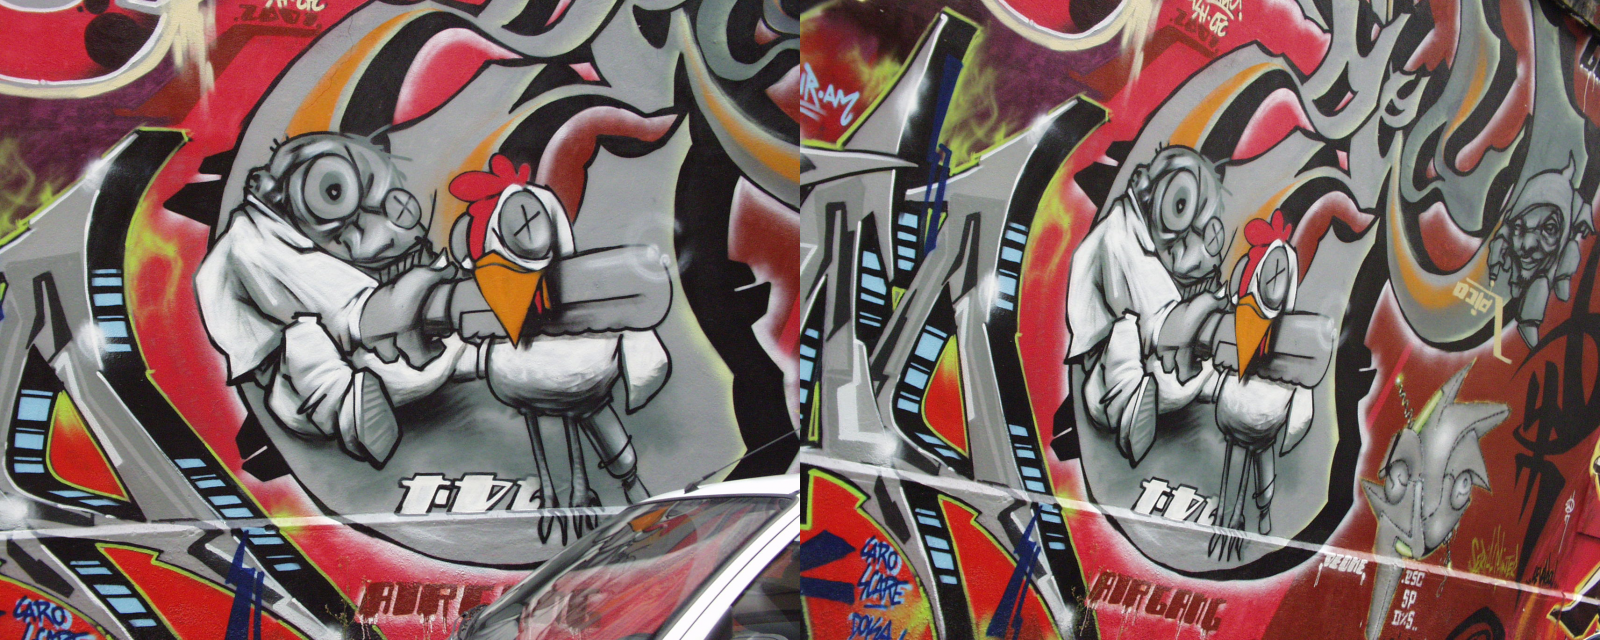
\includegraphics[width=0.75\textwidth]{main/introduction/images/local_features_graffiti.png} \\
%     	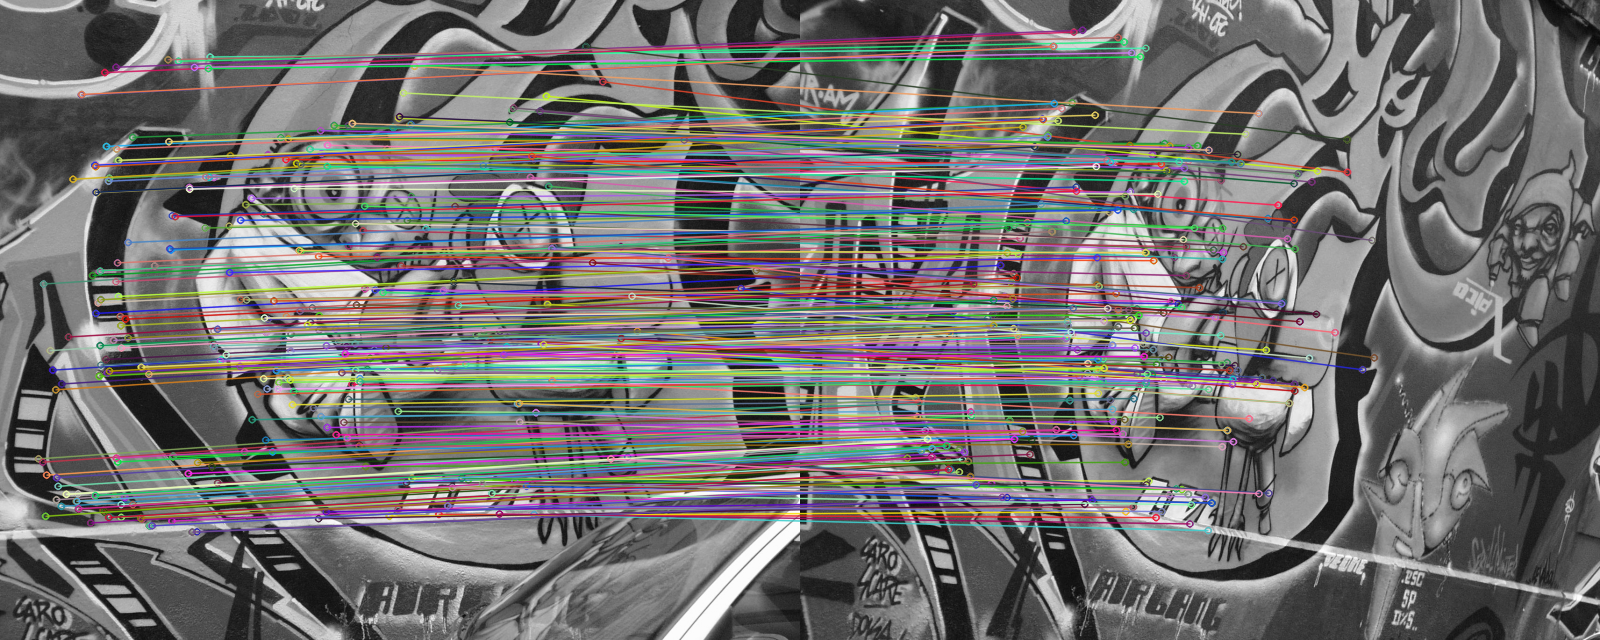
\includegraphics[width=0.75\textwidth]{main/introduction/images/local_features_graffiti_matching.png}
%     \end{tabular}
% 	\caption[Example of the Wide Baseline Stereo algorithm]{\textbf{Example of the Wide Baseline Stereo algorithm.} This figure shows an example for detecting, describing and matching local features. \textbf{Top:} shows the original RGB images of the same scene seen from two different points of view. \textbf{Bottom:} shows the same image in grayscale with the detected keypoints and their correspondences across the two views.}
% 	\label{fig:features_matching_example}
% \end{figure}

\begin{figure}
    \begin{center}
        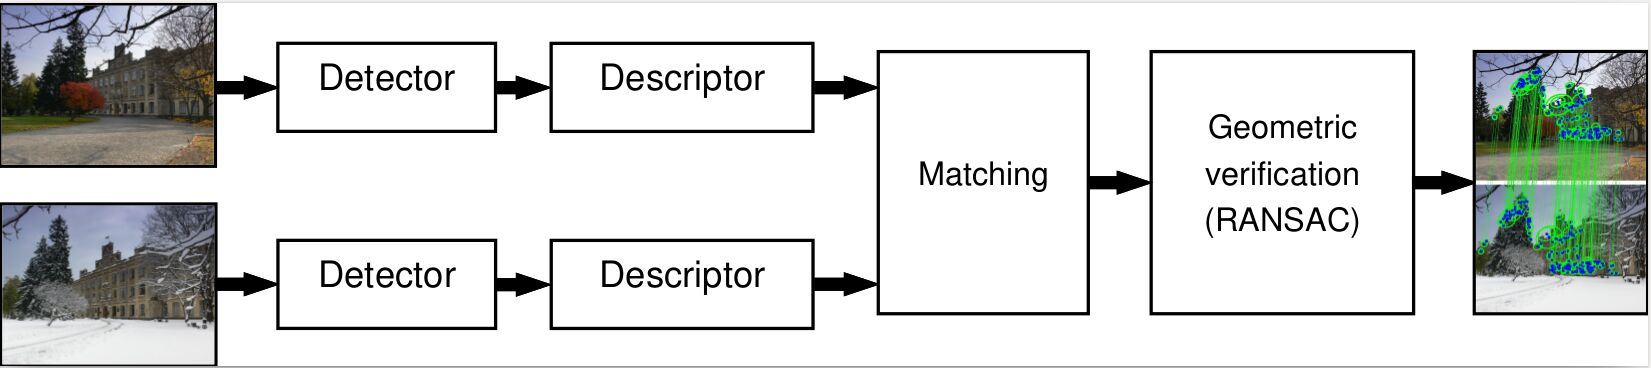
\includegraphics[width=\linewidth]{main/chapter03/data/wbs/wbs_scheme.jpg} 
    \end{center}
    \caption[Wide baseline stereo matching algorithm]{\textbf{Wide baseline stereo matching algorithm.} The diagram of the commonly used wide baseline stereo matching algorithm~\citep{Pritchett1998} that shows the different sub-tasks in the entire pipeline.}
    \label{fig:wbs-pipeline}
\end{figure}

\subsection{Camera Pose Estimation}

% get some inspiration from here: https://ducha-aiki.github.io/wide-baseline-stereo-blog/2020/03/27/intro.html

Choosing the right features to compute the relative pose between two cameras is a crucial task to estimate the depth information of a scene. This can be achieved by the classical process of establishing correspondences between pixels and/or between images and estimating the geometric relation between the cameras. Formally, this process is described as the Wide Baseline Stereo (WBS) algorithm~\cite{Schmid95matchingby} that later can be used as a building block for the application of 3D reconstruction. In figure~\ref{fig:wbs-pipeline} we can see a visual example with the result of the WBS algorithm for the case to align two-images from a different view using the described classical features matching pipeline.
%The different types of features in computer vision can go from detecting edges, corners (or interest points), or blobs (regions of interest points). Every type of feature has its own pros and cons and as we mentioned each application may have different requirements that will make the researchers swing between one or a combination of different features.

As we will see in chapter~\ref{chap:chap_02}, in this thesis we give a strong focus on the detection and description of local features in the context of the WBS algorithm. Thus, in the first place - \textit{What is a local feature?} As stated in~\citep{tuytelaars2008local} a Local Feature can be described as an image pattern which differs from its intermediate neighborhood. Considering that the most common image properties are intensity, color and texture; Local Features can take different forms such as points, edgels or small image patches which can be accompanied by a descriptor vector. Traditionally, local features have been defined using hand-crafted methods~\cite{SIFT, ORB} that allowed to detect singular elements from a single scene across different views in order robustly align the images. However, similar to~\cite{ZagoruykoCVPR2015, detone2017superpoint} in this thesis in chapter~\ref{chap:chap_02} we review and propose new methods for detecting and describing local features based on Convolutional Neural Networks (CNN).

% that later will be converted into descriptors mapping the image properties that we just described. Local Features are a powerful tool that has been successfully used in different applications for instance edge detection in aerial images that often corresponds to roads; blob detection that can be used to identify impurities in some inspection task, etc. Thus, in this thesis we are more interested in the fact that local features can be really relevant as long their location can be determined accurately across different views, see an example in figure~\ref{fig:features_matching_example}. For this same reason, local features are very powerful in applications such as matching or tracking and specially for camera calibration or 3D reconstruction.

% One of the most popular application where the WBS algorithm can be directly applied is in robotics mapping, which typically is the task to create a map based on the information captured by the robot perception system. This problem can be also referred as Simultaneous Localization and Mapping or commonly known as SLAM, which using computational geometry aims to construct and update a map of an unknown environment while simultaneously keep tracking the agent location within it. The classical pipeline for solving SLAM problems based on input images, involves several intermediate steps that can be shared across many other applications. One those intermediate steps, and the one that we will focus more in this thesis, consists in extracting local features, from images that later combined with different geometric techniques can be used to compute either the agent location or for updating the map reconstruction.

\begin{figure}
	\centering
    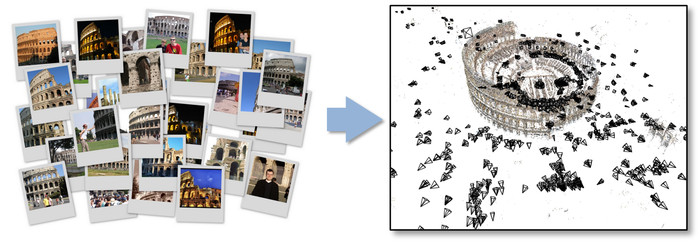
\includegraphics[width=\textwidth]{main/introduction/images/bundler_example.jpg}
    \caption[Structure from Motion example]{\textbf{Structure from Motion example.} This figure shows an example of the result of a Structure from Motion pipeline which reconstructs an entire scene given a set of unordered images. The image is from \textit{Bundler}~\cite{snavely2006}.}
	\label{fig:sfm_example}
\end{figure}

\subsubsection{Structure from Motion}

One of the most popular applications where the camera pose estimation approach can be directly applied is Structure from Motion (SfM)~\cite{ullman1979}. SfM can be described as the technique associated to the field of photogrammetry that tries to estimate a three dimensional representation from two or more images based on the local motion between the different view information (see figure~\ref{fig:sfm_example}). The main principle for SfM is based on the motion parallax theory that using the difference between the displacement of the different views and from the depth information will be used to estimate an accurate 3D representation of the world. Finding the structure from motion it is directly related to stereo vision since in both cases it is needed to have a geometric relation between the different image views.
%This is another sub-problem in the classical pipeline, to find pixel correspondences that relates one pixel from one image to another, typically with sub-pixel precision. The process for finding correspondence is typically solved by extracting local features, and as we mentioned before, can be done using techniques with the same theory background that the ones used for solving visual SLAM problems.

\begin{figure}
    \centering
    \subfloat[\centering]{{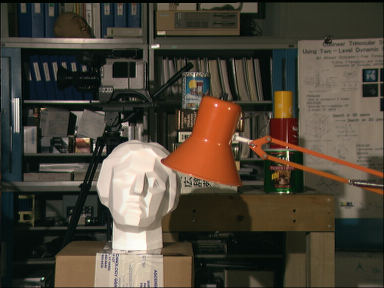
\includegraphics[trim={0 0 0 0.35cm},clip, width=4cm]{main/introduction/images/tsukuba1.png} }}
    \subfloat[\centering]{{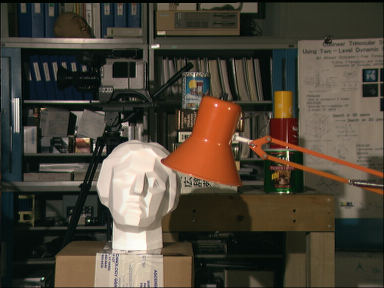
\includegraphics[trim={0 0 0 0.35cm},clip, width=4cm]{main/introduction/images/tsukuba1.png} }}
    \subfloat[\centering]{{
\includegraphics[width=4cm]{main/introduction/images/tsukuba_depth.png} }}
    \caption[Stereo vision system example]{\textbf{Stereo vision system example.} The figure shows a sample from a stereo camera setup from Tsukuba dataset~\cite{PerisMMOF12}. The first two images (a) and (b) correspond to the left and right camera of the setup. The image (c) represents the ground truth depth map of this stereo pair.}
    \label{fig:stereo_example}
\end{figure}

\subsection{Depth Maps Estimation}

In the previous section we introduced how to solve the 3D reconstruction of a scene using as a starting point the estimation of the relative pose between the cameras in order to obtain a sparse reconstruction of the scene. In this section we give a general overview for estimating dense depth maps using stereo systems, range imaging for RGB-D cameras and monocular depth estimation using deep learning methods for the case of multi-camera views.

\subsubsection{Stereo systems}

In classical computer vision exist alternatives for estimating the depth information from a two different views with a known calibration and relative pose which simplifies the problem. These are the stereo systems, which similarly to the human binocular vision system, have two equidistant cameras, displaced horizontally to obtain two different views on a scene. In order to produce the depth information, the stereo systems compare the two images and estimate a disparity, which encodes the difference in horizontal coordinates of the corresponding image points. The values in this disparity map are inversely proportional to the scene depth at the corresponding pixel location (see figure~\ref{fig:stereo_example}). Several works have proposed solutions for stereo matching using classical methods~\cite{boykov2001} that are effective in controlled environments. On the other hand, the stereo matching minimization problem is NP-complete leading sometimes to expensive computational solutions. For this reason, novel approaches based on CNN~\cite{fischer2015flownet, ahmadi2016} methods have been proposed that improve the quality and convergence speed of the stereo vision matching algorithm.

%To work with stereo systems has a lot of pros and cons, since its uses RGB cameras and usually in a calibrated setup which the baseline between the camera is known and helps a lot with the process to solve the depth. However, the use of RGB images can be a bit critical since they are a bit noisy in front of light changes and this might affect the final result of the depth maps.

\begin{figure}
	\centering
    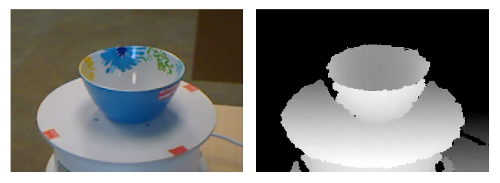
\includegraphics[width=\textwidth]{main/introduction/images/rgbd_kinect.png}
    \caption[Range Imaging example]{\textbf{Range Imaging example.} The figure shows an RGB image (left) and the ground truth depth (right) obtained from a Kinect sensor. This sample is from the RGB-D Object Dataset~\cite{lai2011}.}
	\label{fig:kinect_image}
\end{figure}

\subsubsection{Range Imaging}

A different approach to estimate the depth information of a scene is using range imaging techniques to produce a 2D image containing the distance to points in a scene from a specific 3D point. The resulting image, commonly called range image or depth map contains a distance value for every pixel in the image which with a proper calibration can be directly related to a physical unit (see figure~\ref{fig:kinect_image}).

There are several devices to produce depth maps, usually referred as range cameras or RGB-D cameras that directly produce the depth information of the scene. These type of sensors project a known pattern on the scene by illuminating the scene with a specially designed pattern, structured light, that permit to determine the depth information from the reflected light. These type of devices are extensively used in robotics applications, or in controlled environments since they suffer from the limited measurement range and outdoor sunlight sensitivity~\cite{tateno2017cnnslam}.

% such as structured light or time-of-flight camera which are able to produce already very approximated depth maps. The information obtained from this type of cameras is very valuable for some applications such as in robotics since it solves part of the pipeline for finding the 3d representation of the environment. Range cameras are not the solution to this problem since they are also affected by different lighting conditions and can produce sometimes inaccurate results and artifacts in the predicted depth maps. Recent methods try to solve monocular depth estimation using CNN which produce very challenging results compared to classical methods.
% The mentioned methods are usually computationally expensive in normal scenarios and almost impossible to use in real applications such as in robotics where other high level tasks depend on the perception algorithms.

\subsubsection{Monocular depth estimation}

With the raise of deep neural networks showing their outstanding performance over classical computer vision methods~\cite{He_2017_ICCV, RonnebergerFB15}, recent approaches have been proposed also for the task of depth estimation using convolutional neural networks (CNNs)~\cite{GargBR16}. Additionally, a variety of methods with different architectures have shown that a pixel-level depth can be recovered from a single image in an end-to-end manner based on recurrent neural networks (RNNs)~\cite{abs-1904-07087}, variational auto-encoders (VAEs)~\cite{abs-1902-02086} and generative adversarial networks (GANs)~\cite{aleotti2019}. Following this same direction, in chapter~\ref{chap:chap_05} we propose a novel end-to-end method to estimate the depth information of a scene from different views combining classical geometric computer vision techniques and deep learning.


%A robotics application example is cloth manipulation, a tasks that fully relies on a highly accurate estimation of the 3d shape of the object, see figure~\ref{fig:cloth_manipulation_example}. Many robotics applications still use classical methods such as stereo systems, since RGB cameras are cheap and the algorithms used are very optimised for those platforms, or as described before others can use RGB-D cameras to avoid the cost of computing depth maps. One of the goals for such applications is to get a reconstruction of the scene as much accurate as possible in order to determine different high level task, for example the planning for a the trajectory of a robot arm. It is common that when working with single or even stereo-cameras we suffer from a common problem in vision produced by the motion parallax which is the lack of information from a view, this are referred as occlusions. Having occluded parts in our observations can lead to several problems since it can be one of the reasons for loosing precision and making sometimes difficult to reason for the subsequent tasks. A common solution to solve this issue is include more cameras to the system - this is called mult-view stereo systems that by triangulation methods will complete the missing information. However, for some real applications having more cameras is not feasible, and a natural action would be to move the robot around to explore and complete the missing information from more observations. Another approach would be to provide extra information to the system such as the object mesh, that can be registered with local features and infer the camera pose respect to the object.

% ----------------------------------------------------------------
\newpage
\section{Thesis contributions} 

In this thesis, we analyze the problem of scene reconstruction and we contribute with novel methods for detecting and describing keypoints, a framework that eases the transition from classical to end-to-end deep learning methods, and finally, an end-to-end solution to estimate depth maps using a multi-view camera approach. The rest of this thesis is organised as follows:

\begin{itemize}
    \item In chapter 2, we study the problem of scene reconstruction in the context of the described classical features matching pipeline focusing on the specific tasks to detect and describe local features. The contributions made in this chapter consist of two novel CNN-based modules to be integrated in the traditional scene reconstruction pipeline: a keypoint detector and a keypoint descriptor.
    %we analyze in detail the approach of detecting local features and computing descriptors from the extracted image patches for image matching and 3D reconstruction. In this chapter we will focus on showing how traditional behave respect to CNN based methods and we compare with two proposed solutions - the first that improves a detector based on a geometry loss by learning CNN features, and the second, a shallow CNN that uses a Triplet loss to learn to produce local descriptors that improve previous state of the art methods for feature matching.
    
    \item In chapter 3, we study the integration of classical image processing algorithms within the computational graph of a deep learning system in order to simplify the design of end-to-end pipelines. We contribute with Kornia, a framework that combines classical computer vision with modern auto-differentiable deep learning technologies which makes use of different hardware acceleration capabilities to run the algorithms in the GPUs and TPUs. 
    %we will discuss about the use of mixed methods for classical and learned methods in the Computer Vision field. We provide an extensive review of different methods and applications from the software engineering perspective by proposing a Kornia that combines classical Computer Vision with modern auto-differentiable methods. The chapter will also include several graphical and coding examples about how to use the proposed framework \textit{Kornia} in addition of a review for real applications where the framework can be used for.
    
    \item In chapter 4, we study the problem of scene reconstruction in the context of a multi-camera environment in which we transition from the classic methods to an end-to-end approach. The contribution in this chapters consists in a novel end-to-end CNN-based method that estimates depth maps of deformable objects from an arbitrary camera view exploiting the geometry of the scene.
    %a method to perform view synthesis generation in the context of deformable cloth manipulation for applications where the system requirements makes expensive to include more cameras and reason about the occlusions. We include different experiments using simulated and real data that shows that our system combining deep learned features with classical projective geometry can produce high quality depth maps in front of large rotation angles.
    
\end{itemize}

% ----------------------------------------------------------------
\newpage
\section{First Published Appearances contributions}

The work described in this thesis has been submitted and/or published in different conferences and journals. In the following, the publications related with each chapter are listed:

\begin{itemize}
    \item Chapter 2: Vassileios Balntas, \textbf{Edgar Riba}, Daniel Ponsa, and Krystian  Mikolajczyk. Learning local feature descriptors with triplets and shallow convolutional neural networks. In \textit{BMVC}, 2016.
    \item Chapter 2: Axel Barroso-Laguna, \textbf{Edgar Riba}, Daniel Ponsa, and Krystian Mikolajczyk. Key.Net: Keypoint Detection by Handcrafted and Learned CNN Filters. In \textit{ICCV}, 2019.
    \item Chapter 3: \textbf{Edgar Riba}, Dmytro Mishkin, Daniel Ponsa, Ethan Rublee, and Gary Bradski. Kornia: an Open Source Differentiable Computer Vision Library for PyTorch. In \textit{Winter Conference on Applications of Computer Vision (WACV)}, 2020.
    \item Chapter 3: \textbf{Edgar Riba}, Dmytro Mishkin, Jian Shi, Daniel Ponsa, Francesc Moreno-Noguer, and  Gary Bradski. A survey on Kornia: an Open Source Differentiable Computer Vision Library for PyTorch. In \textit{Journal of Engineering Applications of Artificial Intelligence} (under review).
    \item Chapter 3: Jian Shi, \textbf{Edgar Riba}, Dmytro Mishkin, and Francesc Moreno-Noguer. Differentiable Data Augmentation with Kornia. In \textit{Neurips 2020 Workshop: Workshop on differentiable computer vision, graphics, and physics applied to machine learning}, 2020.
    \item Chapter 4: \textbf{Edgar Riba}, Jordi Sanchez-Riera, Yurun Tian, Fan Zhang, Albert Pumarola, Yiannis Demiris, Krystian Mikolajczyk, and Francesc Moreno-Noguer. Novel View Synthesis of Depth Maps for Cloth Manipulation. In \textit{ICRA} 2021 (under review).
    \item Chapter 4: \textbf{Edgar Riba}, Jordi Sanchez-Riera, Albert Pumarola, Fan Zhang, Yurun Tian, Yiannis Demiris, Krystian Mikolajczyk, and Francesc Moreno-Noguer. Depth Map Synthesis for Deformable Clothes. In \textit{CVPR} 2021 (under review).
\end{itemize}